\subsubsection{UC13 - Inserimento del dizionario dati nel sistema}\label{UC13}

\begin{figure}[H]
  \centering
  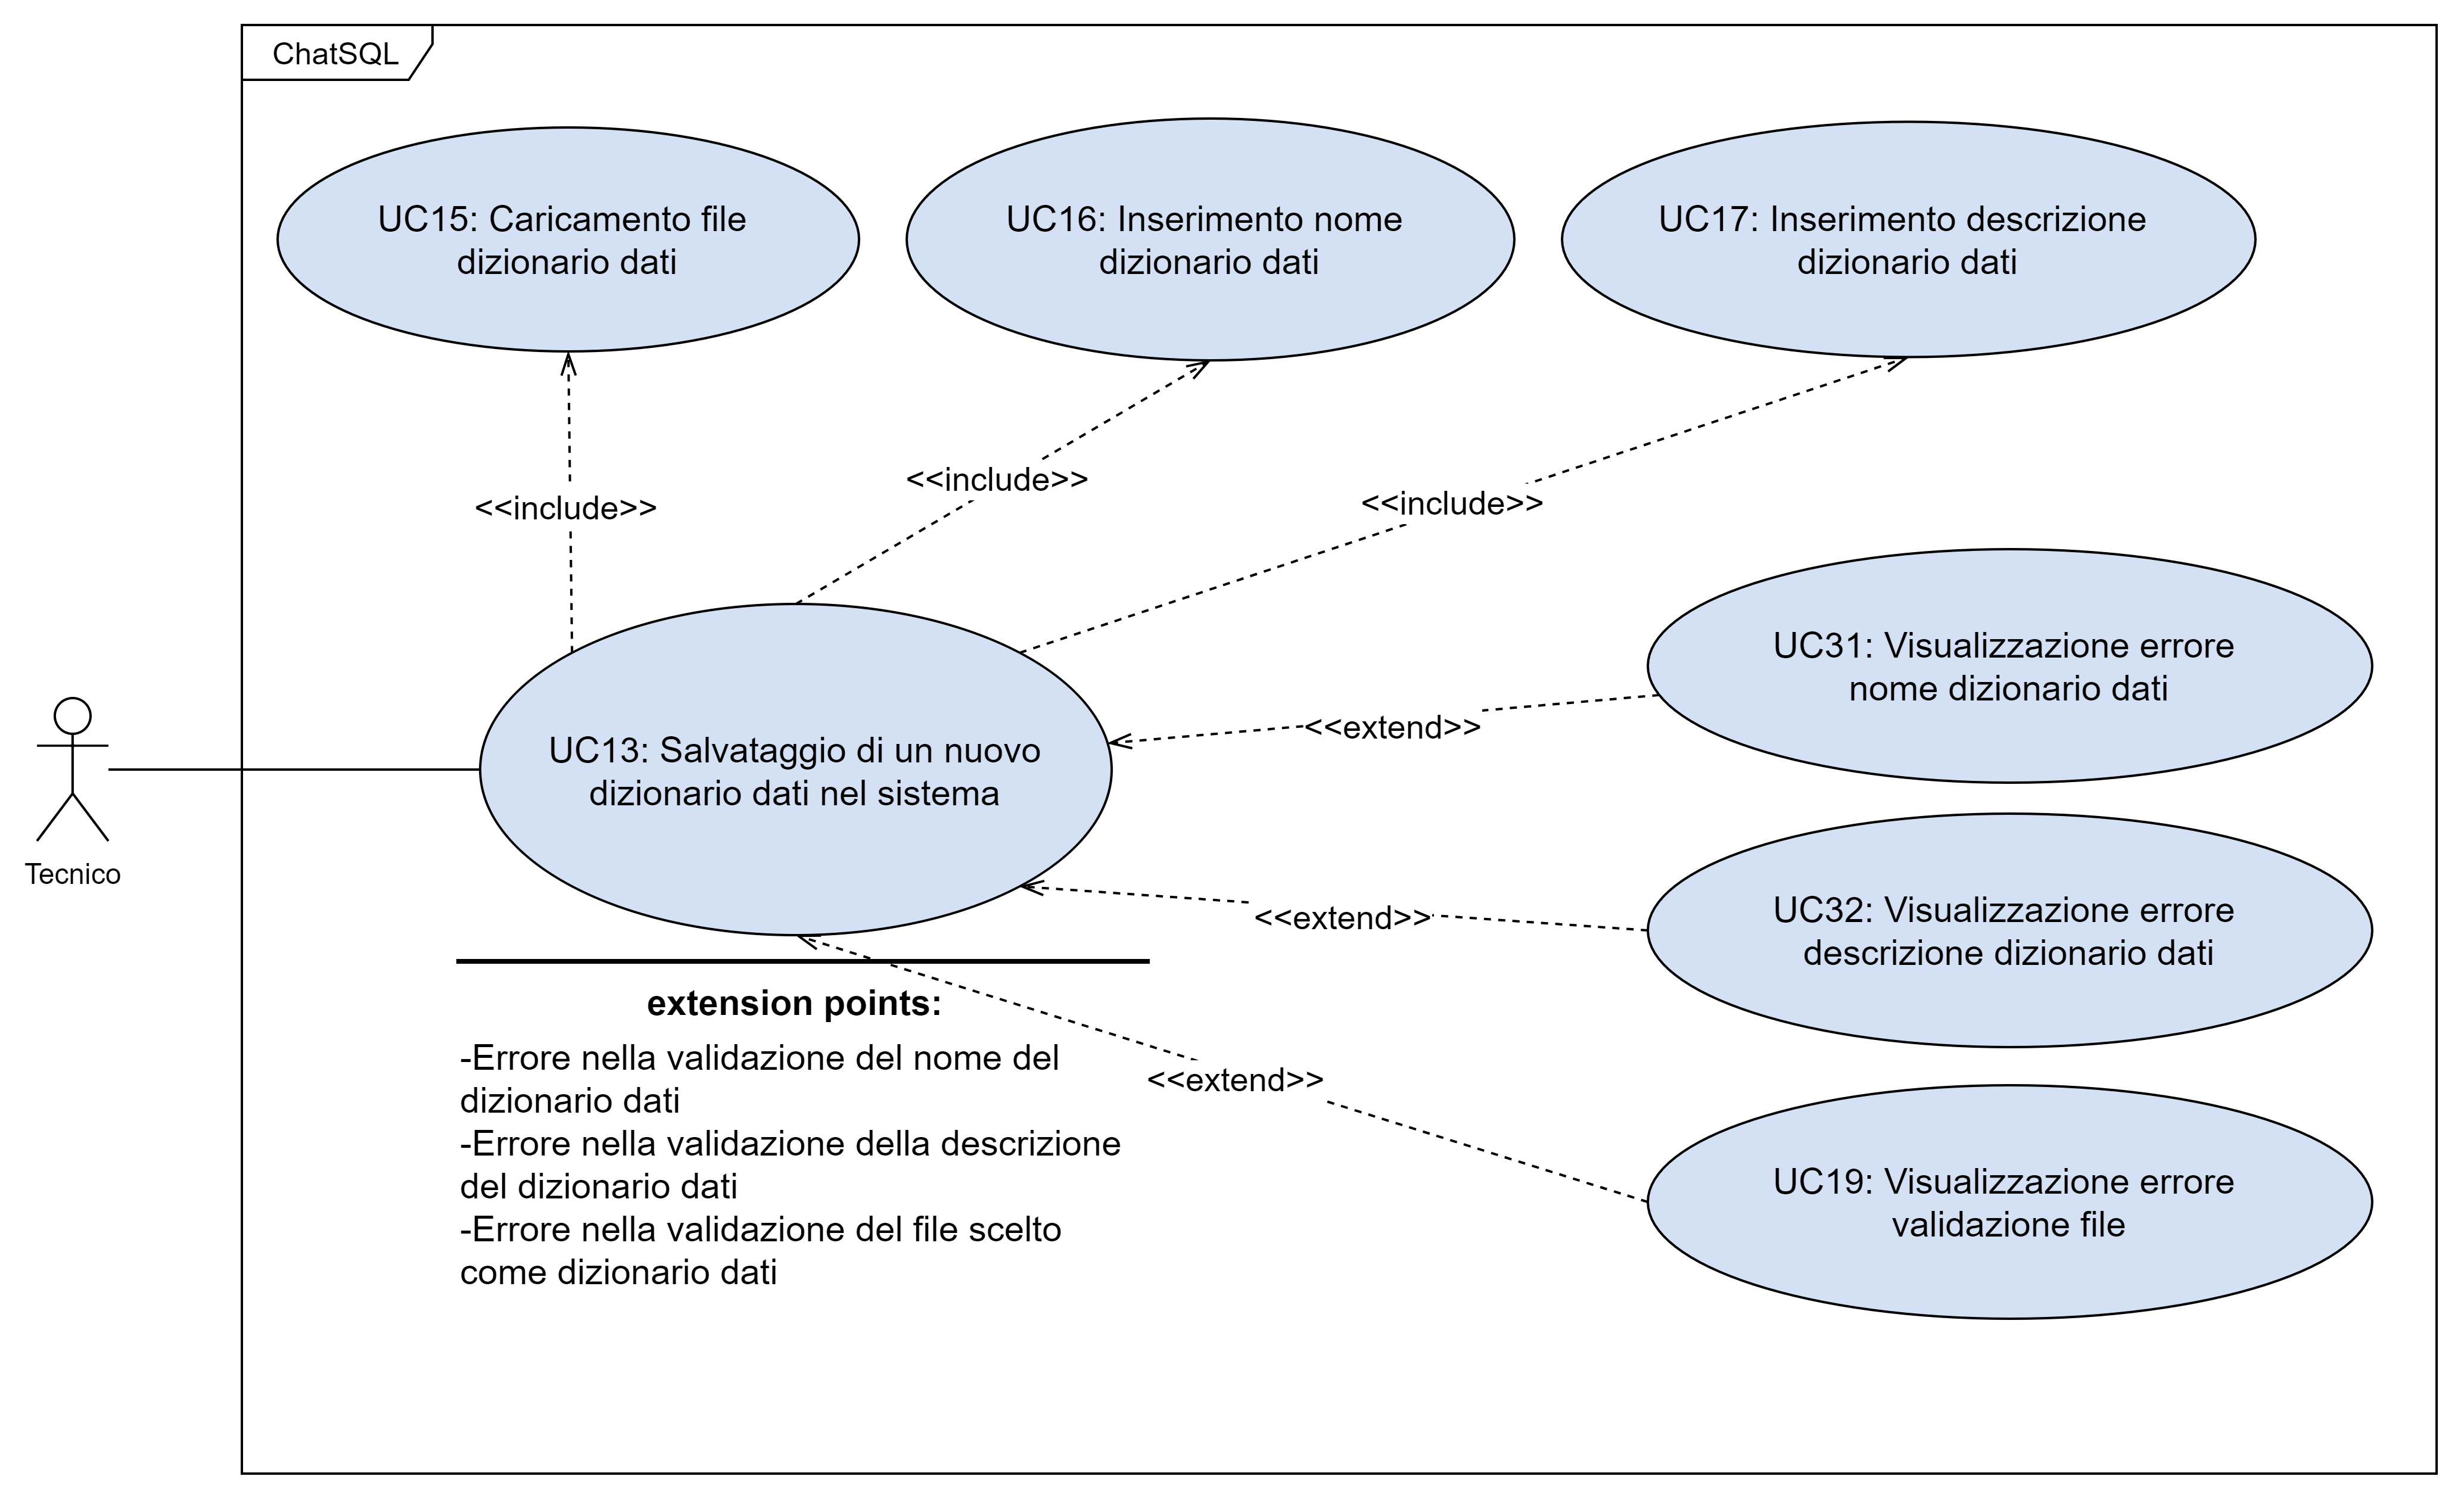
\includegraphics[width=0.90\textwidth]{assets/uc13.png}
  \caption{UC13}
\end{figure}

\paragraph*{Descrizione}
Il salvataggio del \glossario{dizionario dati} corrisponde alla procedura di inserimento di un dizionario e delle sue informazioni all'interno del sistema.

\paragraph*{Attori principali}
Tecnico

\paragraph*{Precondizioni}
\begin{itemize}
  \item Il sistema è attivo e funzionante;
  \item Il Tecnico ha effettuato correttamente l'autenticazione (\hyperref[UC1]{UC1});
\end{itemize}

\paragraph*{Postcondizioni}
\begin{itemize}
  \item Il \glossario{dizionario dati} è stato salvato con successo nel sistema.
\end{itemize}

\paragraph*{Trigger}
Il Tecnico vuole salvare un \glossario{dizionario dati} nel sistema.

\paragraph*{Scenario principale}
\begin{enumerate}
  \item Il Tecnico inserisce il file, il nome e la descrizione del \glossario{dizionario dati};
  \item Viene avviata la procedura di salvataggio del \glossario{dizionario dati};
  \item Il \glossario{dizionario dati} viene aggiunto alla lista dei dizionari presenti nell'applicazione;
  \item Il \glossario{dizionario dati} è ora disponibile a tutti gli utenti e può essere utilizzato per la generazione di \glossario{prompt}.
\end{enumerate}

\paragraph*{Scenario alternativo}
\begin{enumerate}
  \item Il sistema rileva un errore nella validazione del \glossario{dizionario dati} (\hyperref[UC19]{UC19});
  \item Viene visualizzato un messaggio d'errore per il mancato salvataggio del \glossario{dizionario dati}.
\end{enumerate}

\paragraph*{Estensioni}
\begin{itemize}
  \item Visualizzazione errore salvataggio \glossario{dizionario dati} (\hyperref[UC19]{UC19}).
\end{itemize}
